%!TEX root = main.tex
 \section{Current Participant Workflows and Opportunities\label{sec:participantdatasets}}
 %\dor{Given the new subtitles for each domain, not sure if this section title is suitable, since it doesn't encapsulate other aspects such as existing workflows, questions, etc.}
 In this section, we describe our study participants, their scientific goals, and their preferred analysis workflows, based on \rchange{Phase I} of our \cut{design }study.\cut{, where we conducted contextual \rchange{inquiry} to learn about participant's existing workflows.} \cut{We will present findings from our collaborative design process in Section~\ref{sec:pd_findings}.}%, as well as findings from our Phase II evaluation study in Section~\ref{sec:eval_findings}.} %At the start of our design study, we conducted a contextual inquiry to learn about our participants' existing data analysis workflows. 
 While we collaborated with each application domain in depth, we focus on the key findings from each domain to highlight their commonalities and differences, in order to provide a backdrop for our VQS findings described later on. Comparing and contrasting between the diverse set of questions, datasets, and challenges across these three use cases revealed new cross-disciplinary insights essential to better understand how VQSs can be extended for novel and unforeseen use cases.
 %use cases to highlight behaviors that participants have adopted for conducting certain analysis tasks.
 %At the start of our design study, we conducted contextual inquiry to learn about our participants' existing data analysis workflows. Next, we describe our study participants, their scientific goals,  and their preferred analysis workflows.
 % \par\noindent\stitle{Astronomy:} 
 \subsection{Astronomy}
 \par\noindent\stitle{Participants and Goals:} 
 \npar The Dark Energy Survey (DES) is a multi-institution project that surveys 300 million galaxies over 525 nights to study dark energy~\cite{DrlicaWagner2018}. The telescope used to survey these galaxies also focuses on smaller patches of the sky on a weekly interval to discover astronomical transients (objects whose brightness changes dramatically as a function of time), such as supernovae or quasars. Their dataset consisted of a large collection of \emph{light curves}: brightness observations over time, one associated with each astronomical object, plotted as a time series. Over five months, we worked closely with A1, an astronomer on the project's data management team at a supercomputing facility. Their scientific goal was to identify potential astronomical transients in order to study their properties. \cut{These insights can help further constrain physical models regarding the formation of these objects.}
 \par\noindent\stitle{Existing Workflow and Design Opportunities:} 
 \npar \rchange{Since astronomical datasets are often terabytes in scale, they are often processed and stored in highly specialized data management systems in supercomputing centers. First, the astronomer downloads a data sample to explore in a Jupyter notebook, performs data cleaning and wrangling, and verifies data fidelity by computing a set of relevant statistics.} To identify transients, the astronomer programmatically \rchange{generates} visualizations of candidate objects with \texttt{matplotlib} and visually \rchange{examines} each light curve. \rchange{Figure~\ref{CIscreenshot} (left) shows an example of a manually-generated light curve.} If an object of interest \rchange{is} identified through visual analysis, the astronomer may inspect the image of the object for verifying that the significant change in brightness was not due to an imaging artifact. While an experienced astronomer who has examined many transient light curves can often distinguish an interesting transient object from noise by sight, manual searching for transients is time-consuming and error-prone, since the large majority of objects are false-positives. A1 was interested in VQSs as he recognized how specific pattern queries could help astronomers directly search for these rare transients.
 % \par\noindent\stitle{Genetics:}
 \begin{figure}[h!]
   \centering
   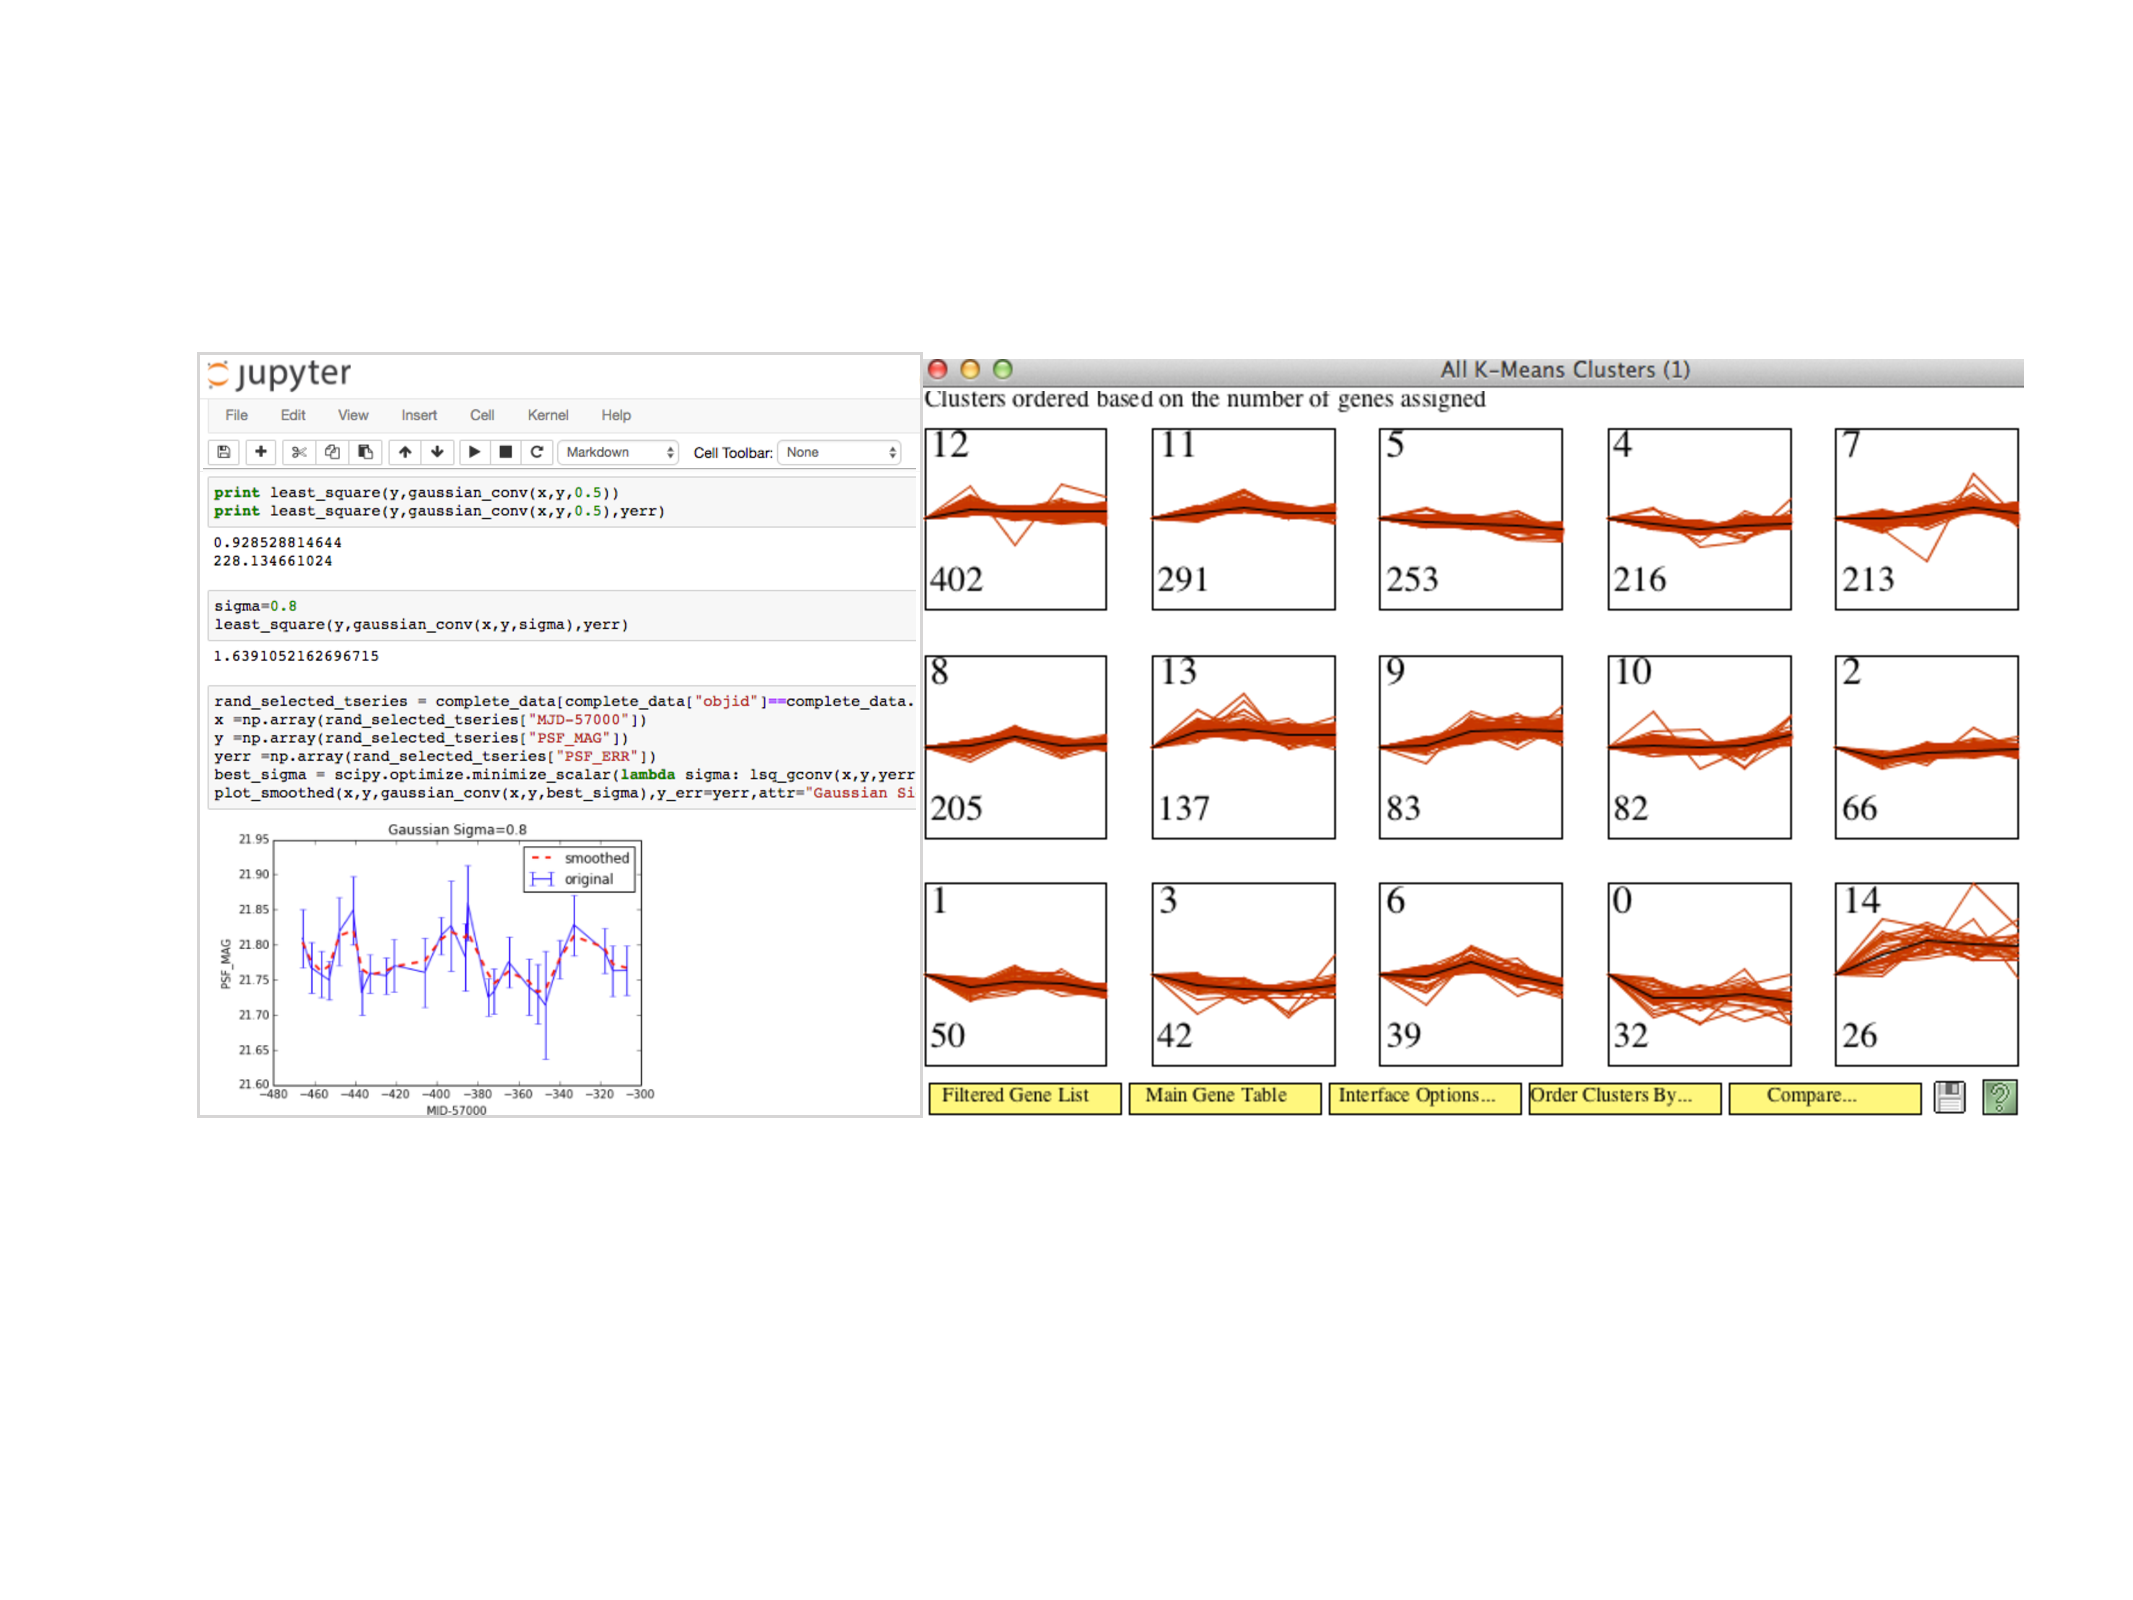
\includegraphics[width=\linewidth]{figures/CIscreenshot.pdf}
   \caption{\rchange{Screenshots from contextual inquiry. Left: A1 performs data smoothing to clean the data and then examines a light curve manually using a Jupyter notebook. Right: G2 uses a domain-specific software to perform clustering and visualize the outputs.}}
   \label{CIscreenshot}
   \vspace*{-20pt}
 \end{figure}
 \subsection{Genetics}
 \par\noindent\stitle{Participants and Goals:} 
 %\techreport{In these experiments, a grid containing thousands of DNA fragments are exposed to stimuli and measurements for the level at which a gene is expressed are recorded as a function of time.} 
 \npar Gene expression is a common measurement in genetics obtained via microarray experiments~\cite{Peng2016}. We worked with a graduate student (G1) and professor (G3) at a research university who were using gene expression data to understand how genes are related to phenotypes expressed during early embryonic development\techreport{\cite{Peng2016,Gloss2017}}. Their data consisted of a collection of gene expression profiles over time for mouse stem cells, aggregated over multiple experiments.
 %\techreport{, downloaded from an online database\footnote{\url{ncbi.nlm.nih.gov/geo/}}. %They were interested in using \zv to cluster gene expression data before conducting analysis with a downstream machine learning workflow.
 % \par\noindent\stitle{Existing Workflow and Design Opportunities:} 
 % \npar Their typical workflow is as follows: G1 first loads the preprocessed gene expression data into a custom desktop application to  visualize and cluster the profiles \footnote{\url{www.cs.cmu.edu/~jernst/stem/}}. After setting several system parameters and executing the clustering algorithm, the overlaid time series for each cluster is displayed on the interface. G1 visually inspects that the patterns in each cluster looks ``clean'' and checks that the number of outlier genes (i.e., those that do not fall into any of the clusters) is low.  If the number of outliers is high or the clustered visualizations look ``unclean'', she reruns the analysis by increasing the number of clusters. Once the visualized clusters look ``good enough'', G1 exports the clusters to her downstream regression tasks.}
 \par\noindent\stitle{Existing Workflow and Design Opportunities:} 
 \npar \rchange{G1 downloads the raw microarray data from a public database and preprocesses the data using a script written in R. G1 then loads the preprocessed gene expression data into custom desktop application to visualize and cluster the gene expression profiles, as shown in Figure~\ref{CIscreenshot} (right).} Prior to the study, G1 and G3 spent over a month \rchange{searching for the optimal number of groups to cluster the profiles, by iteratively tuning the parameters on the clustering application and evaluating the output via a mix of application-provided visualizations and programmatically-generated statistics.}\cut{attempting to determine the best number of clusters for grouping together these gene expression profiles based on a series of statically-generated visualizations and statistics computed after clustering.} While regenerating their results took no more than 15 minutes every time they made a change, the multi-step, segmented workflow meant that all changes had to be done offline.\techreport{, so that valuable meeting time was not wasted trying to regenerate results.} They were interested in VQSs, since interactively querying time series with clustering results had the potential to dramatically speed up their collaborative analysis process.
 %The team were interested in VQSs as they saw how interactively querying time series with clustering results could dramatically speed up their collaborative analysis process.
 %that can improve battery performance and stability
 \subsection{Material Science}
 \par\noindent\stitle{Participants and Goals:} 
 %\par\noindent\stitle{Material Science:} 
 \npar We collaborated with material scientists at a research university who identify solvents for energy-efficient and safe batteries. These scientists worked on a large simulation dataset containing chemical properties for more than 280,000 solvents~\cite{Khetan2018}. Each row of their dataset corresponded to a unique solvent with 25 different chemical attributes. We worked closely with a postdoctoral researcher (M1), professor (M2), and graduate student (M3) to design a sensible way of exploring their data. They wanted to use VQSs to discover solvents that not only have similar properties to known solvents, but are also more favorable (e.g., cheaper or safer to manufacture). To search for these desired solvents, they needed to understand how changes in certain chemical attributes affect other properties under specific conditions.
 \par\noindent\stitle{Existing Workflow and Design Opportunities:} 
 \npar M1 typically \rchange{starts} his data exploration process by iteratively applying filters to a list of potential battery solvents using SQL queries \rchange{(e.g., find solvents with boiling point over 300 Kelvins and lithium solvation energy under 10 kcal/mol)}. Once the remaining solvent list \rchange{is} sufficiently small, he manually \rchange{examines} the properties of each solvent individually by examining the 3D chemical structure of the solvent in a custom software, as well as gathering information regarding the solvent by cross-referencing an external chemical database and existing uses of this solvent in literature. The collected information, including cost, availability, and other physical properties, enabled researchers to select the final set of desirable solvents that could be feasibly experimented with in their lab. They were interested in VQSs as it was impossible for them to uncover hidden relationships between different attributes across large numbers of solvents manually.%(such as how changing one attribute affects another attribute)
 \subsection{\rchange{Themes Emerging From Need-finding Phase}}
 \par \rchange{Across the domains, several themes emerged around the bottlenecks that participants experienced in existing workflows.
 \begin{denselist}
	 \item \textbf{Need for Expressive Querying:} There is often a need to compare amongst large numbers of data instances, yet it is almost impossible to express and search for a desired shape-based pattern through existing programming languages such as SQL and Python.
	 \item \textbf{Need for Integrative Workflows:} Users often switched between preprocessing, parameter specification, code execution, and visualization comparisons. The non-interactive nature of their segmented workflows incurs a large cognitive barrier and hinders collaboration during exploratory data analysis.
	 \item \textbf{Need for Faceted Exploration:} To deal with the large volume of data present, users have to selected particular samples or subsets of data that are ``worth investigating''. Often, the choice of what criteria to apply as filters is also exploratory.
\end{denselist}
 These themes seeded the collaborative feature discovery process, which led to the iterative development of the system prototype, as described next}.
 